\section{Estrutura da Base de Recarga} % (fold)
\label{sec:estrutura_da_base}
	
	O robô terá uma base de recarga automática responsável pelo guiamento do sistema pelo ambiente, pelo recarregamento da bateria e por abrigar e alimentar o Raspberry Pi que fará os cálculos de movimento do sistema.

	\subsection{Solução} % (fold)
	\label{sub:solução}
		
		O requisito é que o robô ao identificar que está com bateria baixa irá seguir para a base seguindo o sinal emitido por ela. A estrutura da base não necessita ter grande porte, por ser fixa e possuir menos equipamentos em seu interior. A base terá uma carcaça quadrada de dimensões 250x250x200mm, como se fosse uma caixa e assim como o robô aspirador, será feito em acrílico ou PVC pela leveza, resistência e custo. Como é uma peça de plástico também evitará condução de corrente, mantendo a proteção do usuário contra choques.  O conector será do tipo magnético, pois no momento em que for ocorrer o encaixe entre as peças do conector, esta possa ser feita de modo mais certeiro e ficará na face oposta à que fica apoiada na parede.

		\begin{figure}[H]
			\centering
			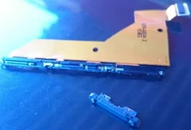
\includegraphics[scale=0.8]{figuras/conector_mag.png}
			\caption{Conectores magnético modelo Sony Xperia.}
			\label{img:conectores}
		\end{figure}

		\begin{figure}[H]
			\centering
			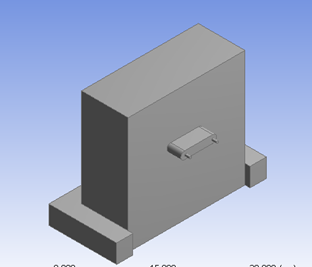
\includegraphics[scale=0.8]{figuras/estrutura_base.png}
			\caption{Estrutura da base de recarga.}
			\label{img:estrutura_base}
		\end{figure}	
	

	% subsection solução (end)
% section estrutura_da_base (end)